
\documentclass[12pt]{article}
 
\usepackage[margin=1in]{geometry} 
\usepackage{amsmath,amsthm,amssymb}
\usepackage{pifont}
\usepackage{graphics}
\usepackage{graphicx}
\usepackage{array}
\usepackage{listings}
\usepackage{matlab-prettifier}

\lstdefinestyle{tex-style} {
	language=Matlab,                           % Code langugage
	basicstyle=\ttfamily,                   % Code font, Examples: \footnotesize, \ttfamily
	%keywordstyle=\color{OliveGreen},        % Keywords font ('*' = uppercase)
	commentstyle=\color{gray},              % Comments font
	numbers=none,                           % Line nums position
	numberstyle=\tiny,                      % Line-numbers fonts
	stepnumber=1,                           % Step between two line-numbers
	numbersep=5pt,                          % How far are line-numbers from code
	%backgroundcolor=\color{gray}, % Choose background color
	frame=single,                             % A frame around the code
	tabsize=2,                              % Default tab size
	captionpos=b,                           % Caption-position = bottom
	breaklines=true,                        % Automatic line breaking?
	breakatwhitespace=false,                % Automatic breaks only at whitespace?
	showspaces=false,                       % Dont make spaces visible
	showtabs=false,                         % Dont make tabls visible
	columns=flexible,                       % Column format
	morekeywords={__global__, __device__}  % CUDA specific keywords
}
\lstset{style=tex-style}
 
\newcommand{\N}{\mathbb{N}}
\newcommand{\Z}{\mathbb{Z}}
 
\newenvironment{theorem}[2][Theorem]{\begin{trivlist}
\item[\hskip \labelsep {\bfseries #1}\hskip \labelsep {\bfseries #2.}]}{\end{trivlist}}
\newenvironment{lemma}[2][Lemma]{\begin{trivlist}
\item[\hskip \labelsep {\bfseries #1}\hskip \labelsep {\bfseries #2.}]}{\end{trivlist}}
\newenvironment{exercise}[2][Exercise]{\begin{trivlist}
\item[\hskip \labelsep {\bfseries #1}\hskip \labelsep {\bfseries #2.}]}{\end{trivlist}}
\newenvironment{problem}[2][Problem]{\begin{trivlist}
\item[\hskip \labelsep {\bfseries #1}\hskip \labelsep {\bfseries #2.}]}{\end{trivlist}}
\newenvironment{question}[2][Question]{\begin{trivlist}
\item[\hskip \labelsep {\bfseries #1}\hskip \labelsep {\bfseries #2.}]}{\end{trivlist}}
\newenvironment{corollary}[2][Corollary]{\begin{trivlist}
\item[\hskip \labelsep {\bfseries #1}\hskip \labelsep {\bfseries #2.}]}{\end{trivlist}}

\newenvironment{solution}{\begin{proof}[Solution]}{\end{proof}}
 
\begin{document}
 
% --------------------------------------------------------------
%                         Start here
% --------------------------------------------------------------
 
\title{Project 1\\
Continuous Time Parameter Estimation Algorithms}
\author{Georgios Kontoudis\\ 
ME6574 Adaptive Control Systems\\
Professor Alexander Leonessa} 
\date{Spring 2018}
 
\maketitle

\begin{question}{1} %theorem, exercise, problem, or question 
\end{question}
The dynamic model and the input are given by
\begin{equation}
m(t)\ddot{y}(t)+\dot{m}(t)\dot{y}(t)=u (t)
\end{equation}
\begin{equation}
u(t)=2\sin(t),
\end{equation}
where the output is the position $y(t)$. The measured signals include noise
\begin{equation}\label{eq_u_noise}
\begin{aligned}
& u_m(t)
& =
&&& u(t)+\epsilon \sin(3t)
\end{aligned}
\end{equation}
\begin{equation}\label{eq_y_noise}
\begin{aligned}
& y_m(t) 
& =
&&& y(t) + \epsilon \sin(3t),
\end{aligned}
\end{equation}
while also the mass drifts
\begin{equation}\label{eq_m_drift}
\begin{aligned}
& m(t) 
& =
&&& 1 + \mu \sin(0.05t).
\end{aligned}
\end{equation}

We derive that state space form 
\begin{equation}\label{eq_stateSpace}
\begin{bmatrix}
\dot{x_1} \\ \dot{x_2}
\end{bmatrix} = \begin{bmatrix}
0 & 1 \\ 0 & -\frac{\dot{m}}{m}
\end{bmatrix} \begin{bmatrix}
x_1 \\ x_2
\end{bmatrix} + \begin{bmatrix}
0 \\ \frac{1}{m}
\end{bmatrix}u.
\end{equation}
Then we apply adaptive laws with projection which reveal
\begin{equation}
Y(s)=W^T(s) \theta^{*}.
\end{equation}
In our case the transfer function, after applying a filter $\Lambda(s)=s^2+12s+7$ with stable poles at $p_1=-3$, $p_2=-4$, yields
\begin{equation}\label{eq_tfW}
W(s) = \begin{bmatrix}
\frac{1}{\Lambda(s)}U(s) \\ 
-\frac{s}{\Lambda(s)}Y(s) \\ 
-\frac{1}{\Lambda(s)}Y(s)
\end{bmatrix}, 
\end{equation}
and the $\theta^*$ vector that we want to estimate takes the form of
\begin{equation}\label{eq_tfWthetaStar}
\theta^* = \begin{bmatrix}
\frac{1}{m} \\ 
-\lambda_1 \\ 
-\lambda_0 
\end{bmatrix}. 
\end{equation}
The block diagram is presented in Figure ... .

Next, we define the error $e_e(t)=w^T(t)\theta(t)-y(t)$ where we will apply the parameter estimation algorithms. For the gradient method we minimize the performance index
\begin{equation}
\min_{\theta(t)} J(t) = \frac{1}{2} e_e^2(t).
\end{equation} 
After differentiation we obtain the update gradient method law
\begin{equation}
\dot{\theta} = -g I w(t)e_e(t),
\end{equation} 
where g is a positive constant value $g \in \mathbb{R}^+$.

For the least squares method we minimize the performance index
\begin{equation}
\min_{\theta(t)} J(t) = \int_0^t e_e^2(\tau) d\tau
\end{equation} 
After differentiation we obtain the time varying scaling matrix update law
\begin{equation}
\dot{P}(t) = -P(t) w(t)w^T(t)P(t),
\end{equation} 
and the update least squares method law
\begin{equation}
\dot{\theta}(t) = -P(t) w(t)e_e(t),
\end{equation}

For the least squares method with forgetting factor we minimize the performance index
\begin{equation}
\min_{\theta(t)} J(t) = \int_{0}^{t} e^{-\lambda (t-\tau)} e_e^2(\tau) d\tau
\end{equation} 
After differentiation we obtain the time varying scaling matrix update law
\begin{equation}
\dot{P}(t) = \lambda P(t)-P(t) w(t)w^T(t)P(t),
\end{equation} 
and the update least squares with forgetting factor method law
\begin{equation}
\dot{\theta}(t) = -P(t) w(t)e(t),
\end{equation}
where $\lambda$ is a positive constant value $\lambda \in U$, $U=\{x\in \mathbb{R}|x\leq 0, x \geq 1\}$.

The MATLAB function is provided bellow.
\begin{lstlisting}
function Xdot = estimation(t,x)
global  lambda r mu m epsilon technique g lambda1 lambda0
M=m+mu*sin(0.05*t); % Mass function
dM=0.05*mu*0.05*cos(0.05*t); % Mass derivative
A = [0 1; 0 -dM/M]; % State matrix
B = [0; 1/M]; % Input matrix
X = [x(1) x(2)]'; % States
u = 2*sin(t); % Input
dx = A*X+B*u; % State space 
y = x(1); % Output
P = [x(3) x(4) x(5); x(6) x(7) x(8); x(9) x(10) x(11)];%Least squares states
Theta = [x(12) x(13) x(14)]'; % Theta states (we want to find this)
um = u + epsilon*sin(3*t); % Input measurement noise
ym = y + epsilon*sin(3*t); % Output measurement noise

% Transfer Function to State Space
X_tf2ss = [x(15) x(16)]';
A_tf2ss = [0 1; -lambda1 -lambda0];
B_tf2ss = [0 1]';
dX_tf2ss = A_tf2ss*X_tf2ss+B_tf2ss*um;
X_tf2ss2 = [x(17) x(18)]';
dX_tf2ss2 = A_tf2ss*X_tf2ss2+B_tf2ss*ym;
W(1) = X_tf2ss(1); % Input measurement filter output
W(2) = -X_tf2ss2(2); % Output measurement filter output 1
W(3) = -X_tf2ss2(1); % Output measurement filter output 2
W=[W(1) W(2) W(3)]'; % Measurements filter outputs
% Update Laws
k=1;
for i=1:3
    for j=1:3
        dP(k) = lambda*P(i,j)-P(i,:)*W*W'*P(:,j); %  LS derivative
        k=k+1;
    end
end
Pr=reshape(P,[3,3])';
if technique==1
    G=g*ones(3,3); % Gain matrix
    dTheta=-G*W*(W'*Theta-ym); % Theta derivative least squares estimation
else
    dTheta=-Pr*W*(W'*Theta-ym); % Theta derivative grad. descent estimation
end
Xdot=[dx;dP';dTheta;dX_tf2ss;dX_tf2ss2;dM];
end
\end{lstlisting}
The MATLAB source file is provided bellow.
\begin{lstlisting}
% Parameters
global lambda r mu m epsilon technique g lambda1 lambda0
technique=2; % 1 for gradient descent, 2 for least squares,  
             % 3 for ls w/forgettings factor
             
noise=2; % 1 for noise-free, 2 for measurement noise, 3 for drift mass,
         % 4 for drift mass and measurement noise
         
% Filter values
lambda0 = 12; 
lambda1 = 7; 
p=[1 lambda1 lambda0];
r=roots(p); % poles in the left plane at -3 and -4 (stable)
alpha = 1987; % initialize least squares matrix P (large value)
m = 1; %mass

% Estimation Cases
switch technique
    case 1 % gradient descent
       lambda = 0; % forgetting factor 
       g=50; % Fixed gain
    case 2 % least squares
       lambda = 0; % forgetting factor 
    case 3 % least squares with forgetting factor
       lambda = .5; % forgetting factor
end

% Noise Inputs
switch noise
    case 1 % noise-free
        mu = 0; 
        epsilon = 0;
    case 2 % measurements noise
        mu = 0; 
        epsilon = 2;
    case 3 % drift mass
        mu = 3; 
        epsilon = 0;
    case 4 % drift mass and measurement noise
        mu = 3;
        epsilon = 2;
end

% ODEs 
x0=[1 2]';
p0=alpha*eye(3);
P0=reshape(p0,[9,1]);
Theta0=[4 1 2]';
M0=2;
x0_tf2ss= [0 0 0 0]'; % Set it to zero, otherwise blows up
x_init=[x0;P0;Theta0;x0_tf2ss;M0];
t_int = [0 20];
options = odeset('OutputFcn',@odeplot); % , 'OutputSel',[1 2] 
[t,x]= ode45(@estimation, t_int, x_init, options);
hold on;

% Plots
[tr,tc]=size(t);
for i=1:tr
    m_desired(i,1) = m;
end
figure (2)
plot(t, x(:,12), 'LineWidth',2);
hold on;
plot(t,m_desired,'--', 'LineWidth',2, 'Color', 'r');
hold on;
set(gca,'FontSize',16);
hold on;
grid on;
ylabel('Estimation of 1/m [kg^{-1}]');
% No drift 'Estimation of 1/m [kg^{-1}]' or 
% Drift mass: 'Estimation of $\dot{m}/m$ [$kg^{-1}$]', 'interpreter','latex'
xlabel('Time [s]');
\end{lstlisting}



\begin{question}{2} %theorem, exercise, problem, or question
\end{question}
Simulations were performed to evaluate the efficacy of the adaptive estimation algorithms. Except of the mass, we evaluate the $b_0$ for all cases. This factor $b_0$ is the ratio $\frac{1}{m}$ that when crosses the zero value, the mass estimation takes large values and as a result the representation is unclear. If the true mass value was not that close to zero, we could depict the estimated value. Moreover, for mass $m=1$ the fraction $\frac{1}{m}=m=1$ has the same value. The estimated parameters $\frac{1}{m}$ and $m$ without noise of all three adaptive estimation methods are depicted in Figure~\ref{fig_noiseFree} and \ref{fig_noiseFree_m} respectively. The estimated parameters $\frac{1}{m}$ and $m$ with measurement errors of all three adaptive estimation methods are illustrated in Figure~\ref{fig_noiseMeasurement} and \ref{fig_noiseMeasurement_m} respectively. The estimated parameters $\frac{1}{m}$ and $m$ with drift mass of all three adaptive estimation methods are presented in Figure~\ref{fig_noiseDrift} and \ref{fig_noiseDrift_m} respectively. The estimated parameters $\frac{1}{m}$ and $m$ with measurement errors and drift mass of all three adaptive estimation methods are shown in Figure~\ref{fig_noise} and \ref{fig_noise_m} respectively. 

\begin{figure}[!h]
	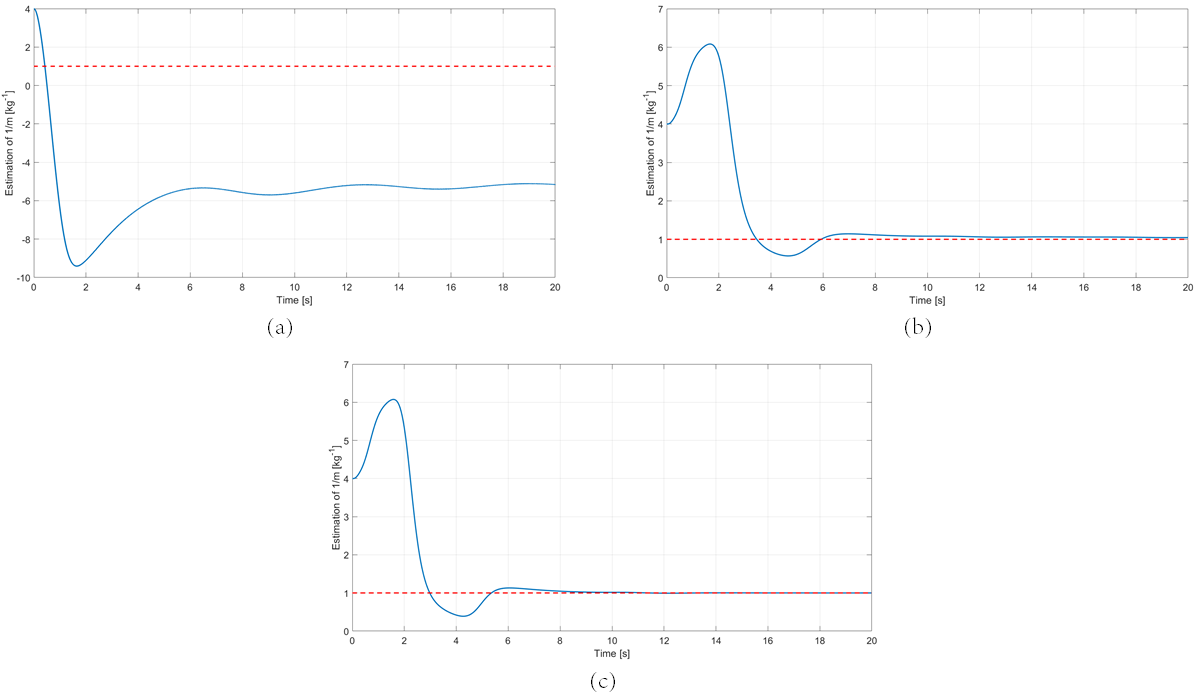
\includegraphics[width=.95\columnwidth]{figures/noiseFree.png}
	\centering
	\caption{The adaptive estimation of the fraction $\frac{1}{m}$ without any noise, a. The gradient method, b. The least squares method, c. The least squares with forgetting factor $\lambda=0.5$.}
	\label{fig_noiseFree}
\end{figure}

\begin{figure}[!h]
	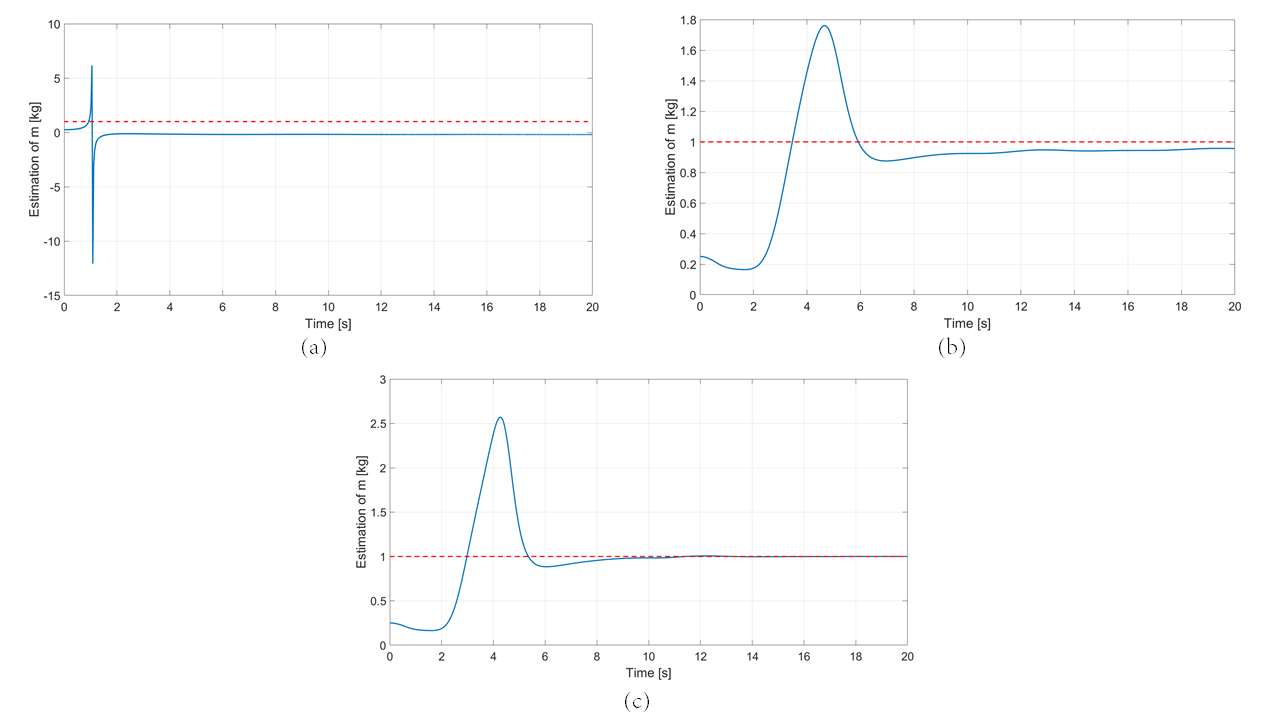
\includegraphics[width=1\columnwidth]{figures/noiseFree_m.png}
	\centering
	\caption{The adaptive estimation of the mass $m$ without any noise, a. The gradient method, b. The least squares method, c. The least squares with forgetting factor $\lambda=0.5$.}
	\label{fig_noiseFree_m}
\end{figure}

\begin{figure}[!h]
	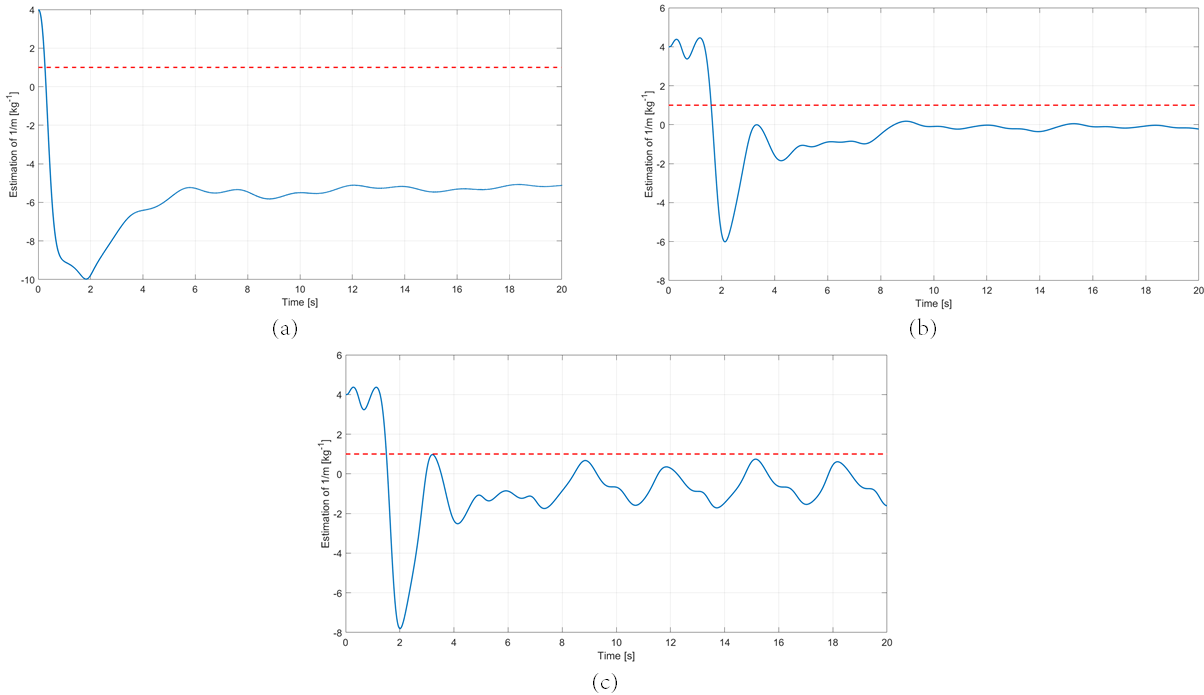
\includegraphics[width=.95\columnwidth]{figures/measurementNoise.png}
	\centering
	\caption{The adaptive estimation of the fraction $\frac{1}{m}$ with measurement noise, a. The gradient method, b. The least squares method, c. The least squares with forgetting factor $\lambda=0.5$.}
	\label{fig_noiseMeasurement}
\end{figure}

\begin{figure}[!h]
	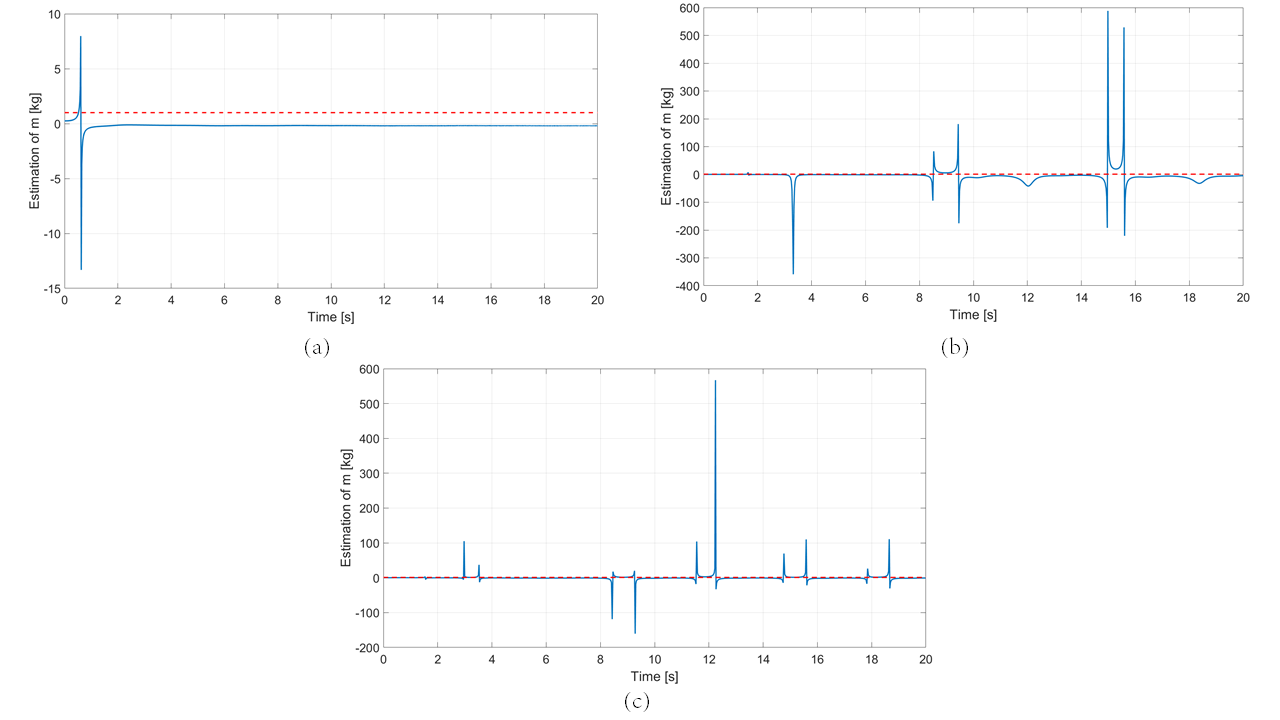
\includegraphics[width=1\columnwidth]{figures/measurementNoise_m.png}
	\centering
	\caption{The adaptive estimation of the mass $m$ with measurement noise, a. The gradient method, b. The least squares method, c. The least squares with forgetting factor $\lambda=0.5$.}
	\label{fig_noiseMeasurement_m}
\end{figure}
 
\begin{figure}[!h]
	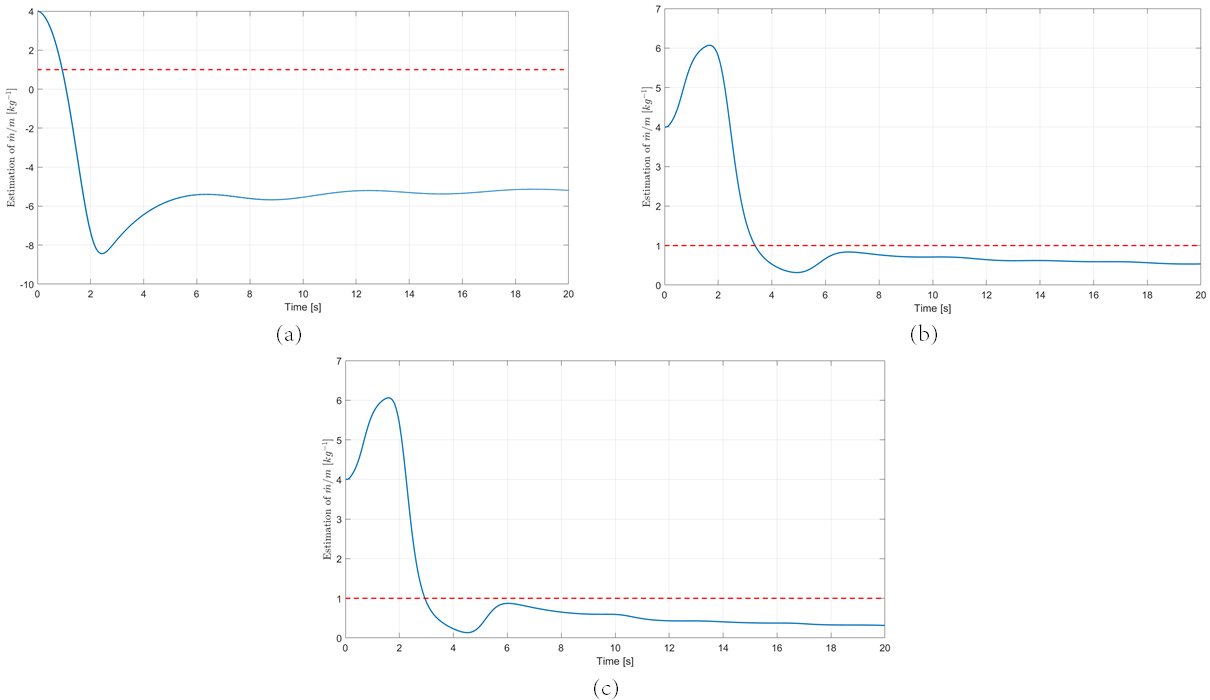
\includegraphics[width=.95\columnwidth]{figures/driftMass.png}
	\centering
	\caption{The adaptive estimation of the fraction $\frac{1}{m}$ with mass drift, a. The gradient method, b. The least squares method, c. The least squares with forgetting factor $\lambda=0.5$.}
	\label{fig_noiseDrift}
\end{figure}

\begin{figure}[!h]
	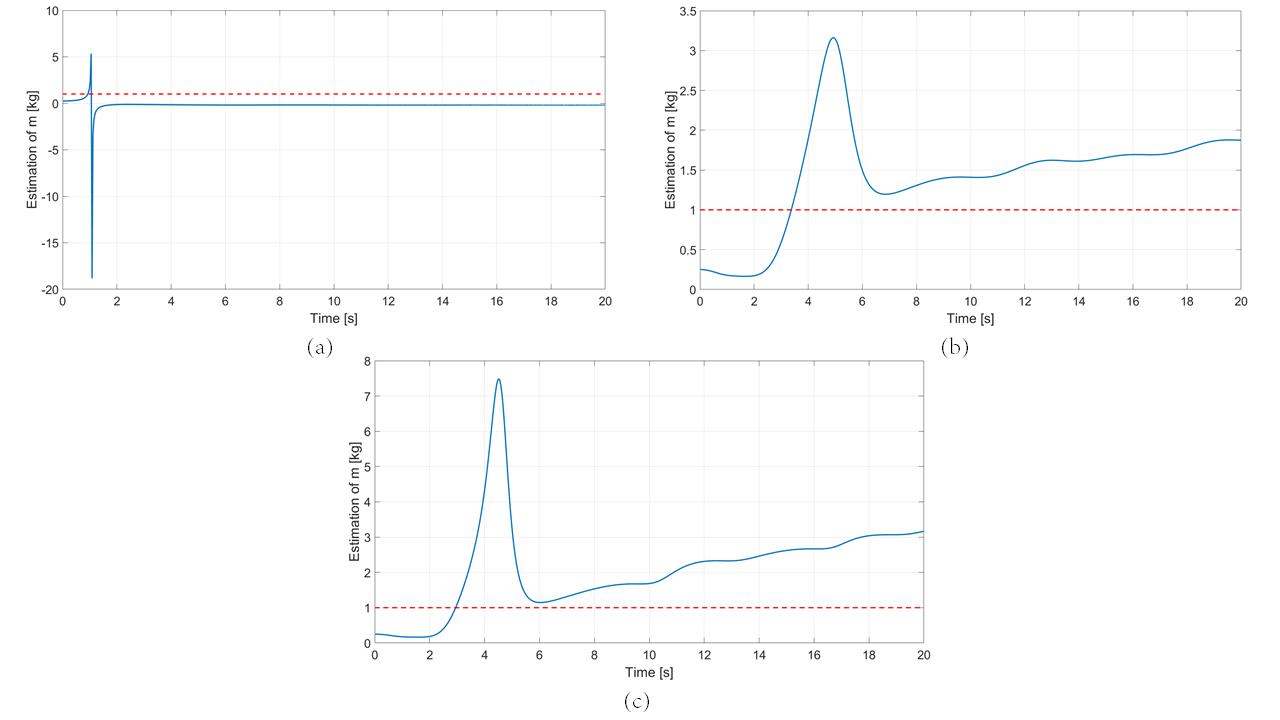
\includegraphics[width=1\columnwidth]{figures/driftMass_m.png}
	\centering
	\caption{The adaptive estimation of the mass $m$ with mass drift, a. The gradient method, b. The least squares method, c. The least squares with forgetting factor $\lambda=0.5$.}
	\label{fig_noiseDrift_m}
\end{figure}


\begin{figure}[!h]
	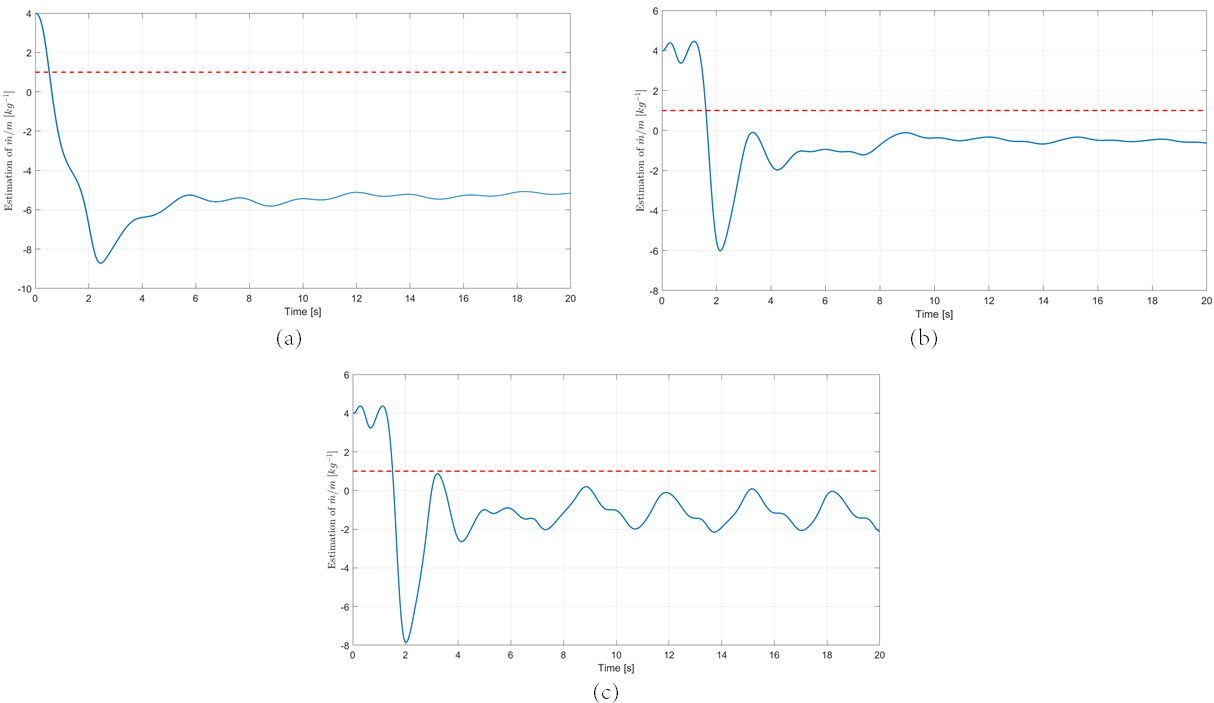
\includegraphics[width=.95\columnwidth]{figures/noise.png}
	\centering
	\caption{The adaptive estimation of the fraction $\frac{1}{m}$ with mass drift and measurement noise, a. The gradient method, b. The least squares method, c. The least squares with forgetting factor $\lambda=0.5$.}
	\label{fig_noise}
\end{figure}

\begin{figure}[!h]
	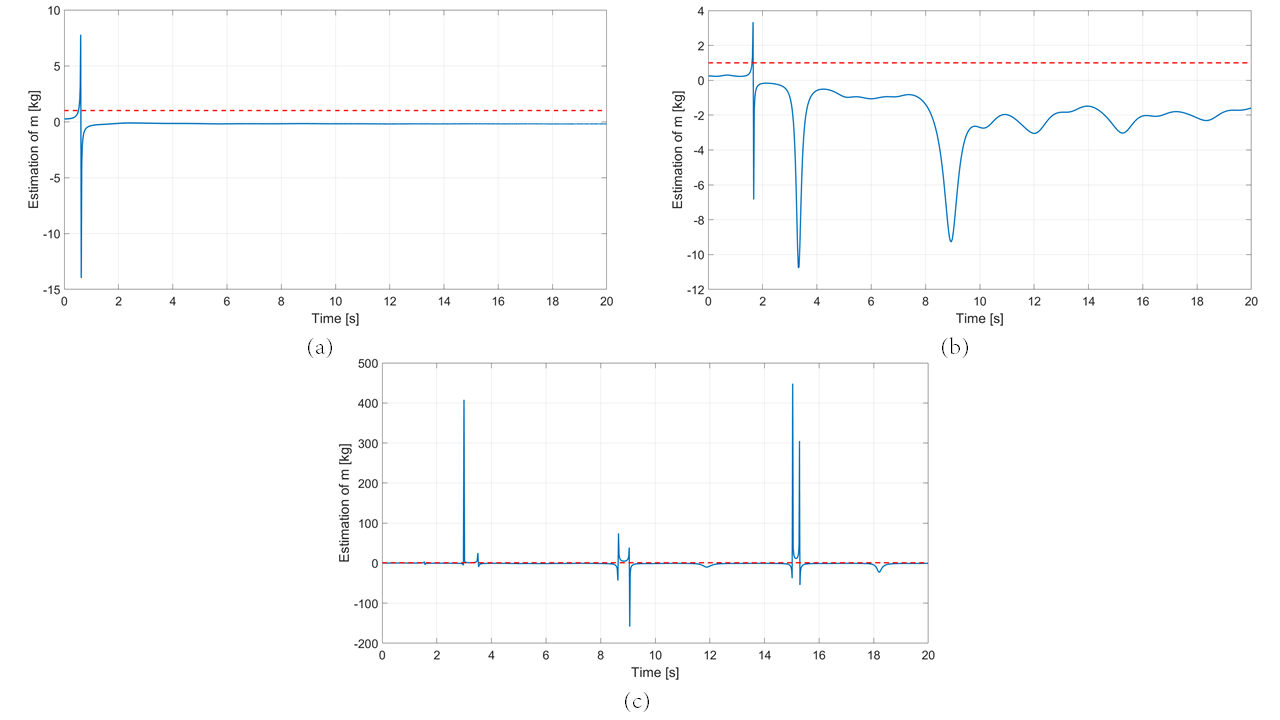
\includegraphics[width=.95\columnwidth]{figures/noise_m.png}
	\centering
	\caption{The adaptive estimation of the mass $m$ with mass drift and measurement noise, a. The gradient method, b. The least squares method, c. The least squares with forgetting factor $\lambda=0.5$.}
	\label{fig_noise_m}
\end{figure}



\begin{question}{3} %theorem, exercise, problem, or question 
In case that no noise or mass drift appears in the system then the least squares estimation with forgetting factor has the best performance as presented in Figures~\ref{fig_noiseFree} and \ref{fig_noiseFree_m}. The least square estimation has similar performance, yet it doesn't converge in the correct value and maintains a small error at steady state. The gradient estimation algorithm has a large error, because we are not driving the gain matrix $G$ to zero. In Figure~\ref{fig_noise_variousG} we evaluate various gain values, which indicates that the error is not related with the initial gain value $G$. Moreover, the overshoot increases along with the gain propagation.

\begin{figure}[!h]
	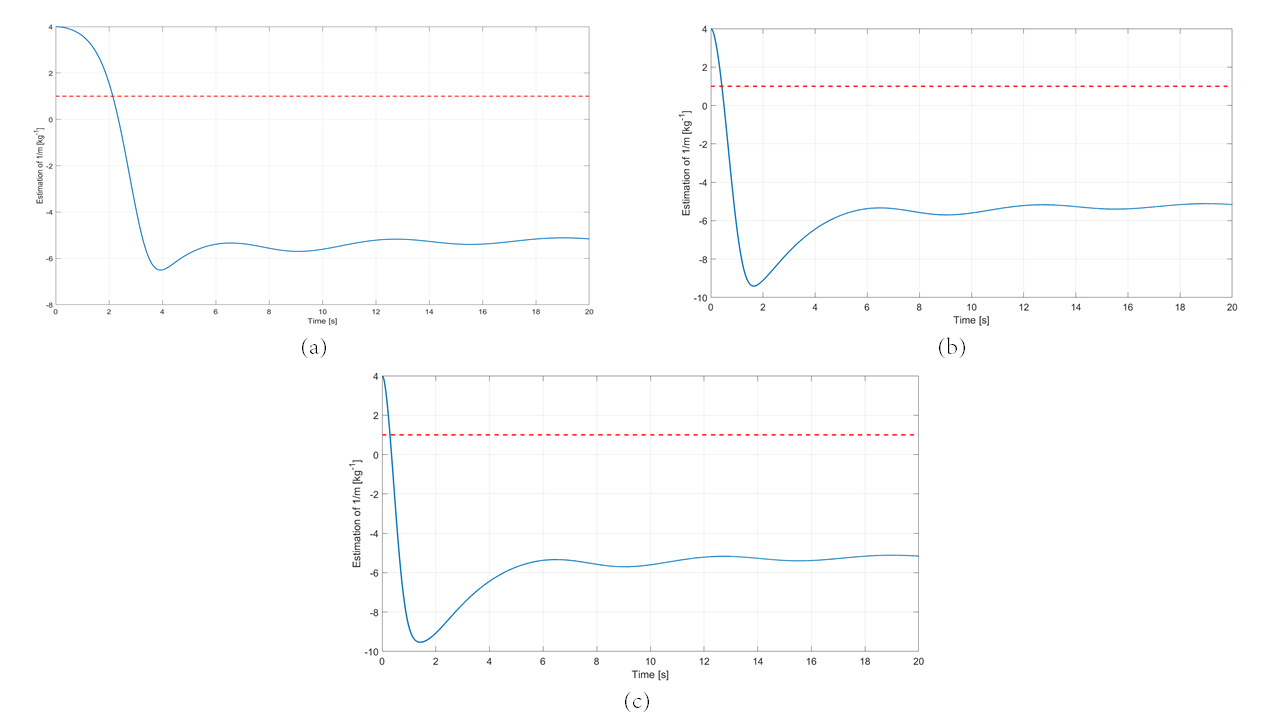
\includegraphics[width=.95\columnwidth]{figures/gradient_noiseFree_variousgG.png}
	\centering
	\caption{The gradient estimation method of the $\frac{1}{m}$ without noise and various gains, a. With gain $g=1$, b. With gain $g=10$, c. With gain $g=100$.}
	\label{fig_noise_variousG}
\end{figure}

On the other hand the initial conditions affect the error that appears in the gradient estimation method as depicted in Figure~\ref{fig_noise_variousx0}. More precisely we could potentially estimate the correct value but only when starting at a specific initial condition.

\begin{figure}[!h]
	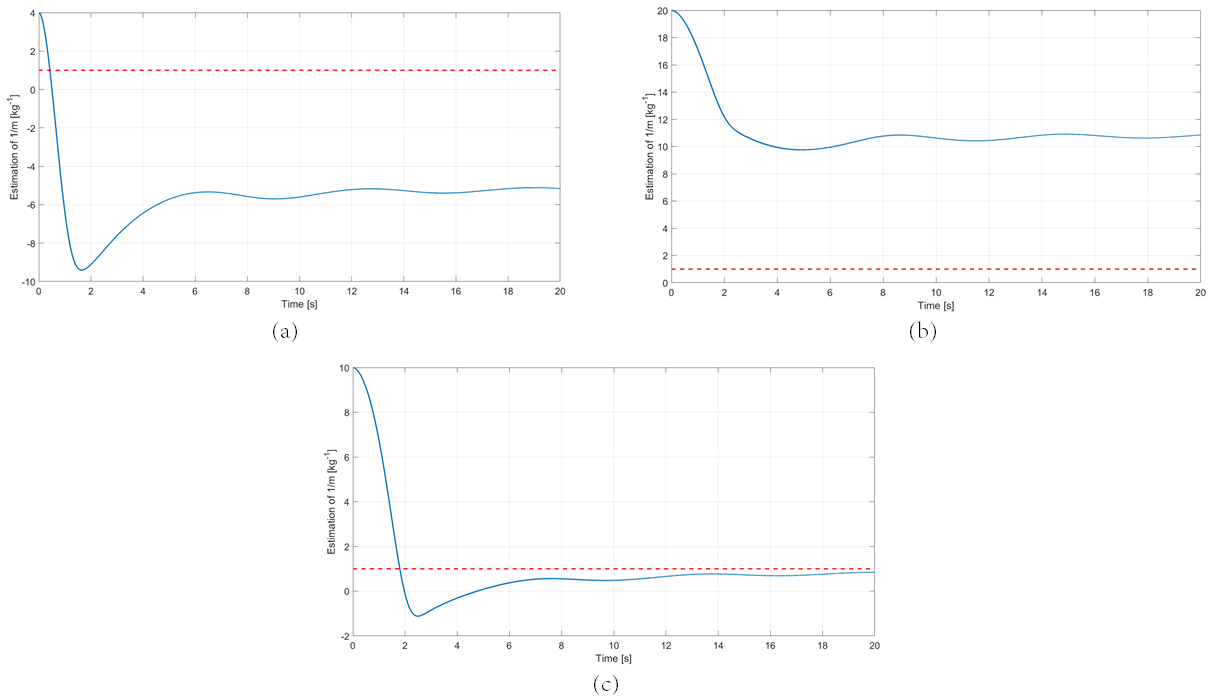
\includegraphics[width=.95\columnwidth]{figures/gradient_noiseFree_variousgx0.png}
	\centering
	\caption{The gradient estimation method of the $\frac{1}{m}$ without noise and various initial conditions, a. Starting at $y=4$, b. Starting at $y=20$, c. Starting at $y=10$.}
	\label{fig_noise_variousx0}
\end{figure}

For the case of sensor measurements noise, the least squares estimation has the best performance as shown in Figures~\ref{fig_noiseMeasurement} and \ref{fig_noiseMeasurement_m}. Yet it cannot reach the correct value. The least square estimation method with forgetting factor appears many oscillation, but the mean value stays the same with the least square estimation method. The oscillations are periodic and appear due to the forgetting of previous information. More specifically the values of the scale matrix $P$ are oscillating around 0, because of the the forgetting factor. Note that if we increase the forgetting factor to $1$ the magnitude of the oscillations increases, while if we set it to zero it is the same with the least square estimation method as presented in Figure~\ref{fig_forgettingMeasurement_various_lambda}.

\begin{figure}[!h]
	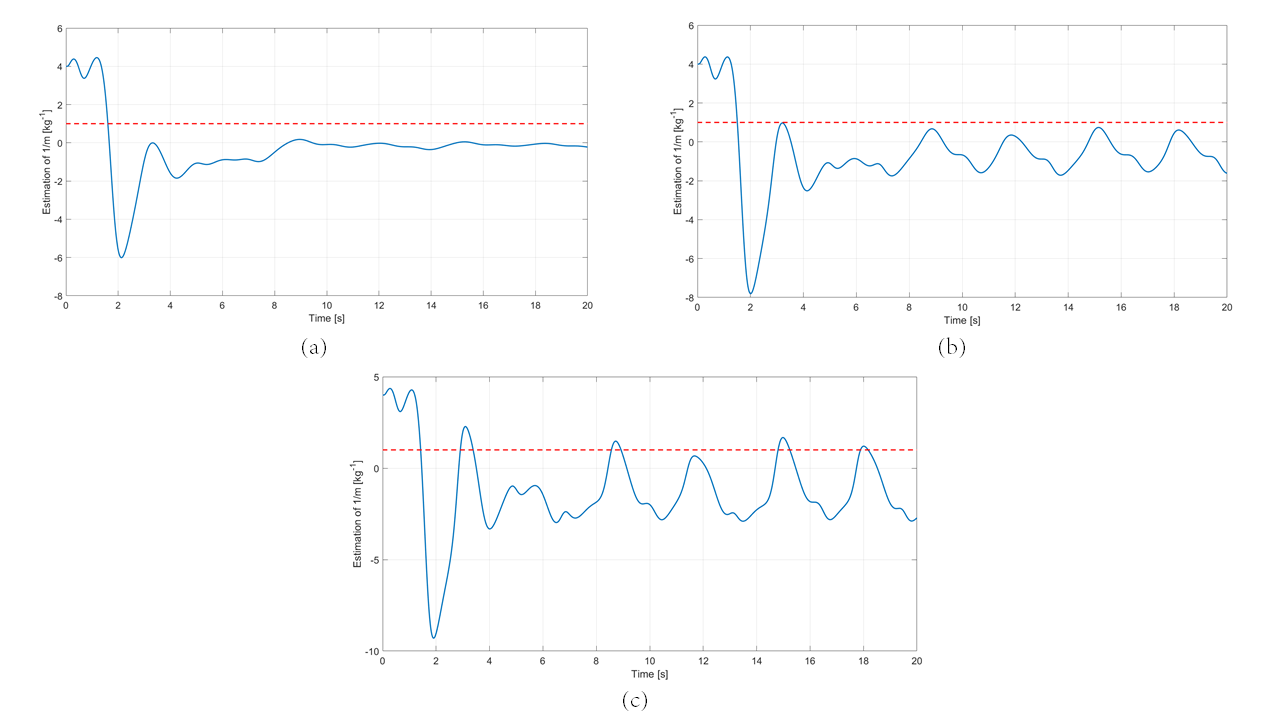
\includegraphics[width=.95\columnwidth]{figures/LS_forgetting_various_lambda.png}
	\centering
	\caption{The gradient estimation method with forgetting factor of the $\frac{1}{m}$ with measurement noise, a. Forgetting factor $\lambda=0$, b.Forgetting factor $\lambda=0.5$, c. Forgetting factor $\lambda=1.0$.}
	\label{fig_forgettingMeasurement_various_lambda}
\end{figure}
\end{question}

The least squares estimation has the best performance on mass drift as shown in Figures~\ref{fig_noiseDrift} and \ref{fig_noiseDrift_m}. Yet it maintains an small steady state error which increases through time. The error propagation occur because the approximation the scale matrix $P$ has been driven to zero and the dynamics are changing through time, so it cannot affect the estimation algorithm. The same applies to the least squares estimation with forgetting factor, but the error is also amplified due to the forgetting factor. This happens because we loose previous information which indicates that the effect of the scale matrix $P$ is artificially reduced. The gradient estimation method it maintains the large error, yet it tracks the effect of drift mass since $G$ is a constant matrix.

For the case of both mass drift and measurement noise the least squares estimation has the best performance as shown in Figures~\ref{fig_noise} and \ref{fig_noise_m}. We have the same characteristics of drift mass along with the measurement noise. More specifically the drift mass increase the steady state error through time and the measurement noise add oscillations to the system. 

\begin{question}{4}\end{question}
For the adaptive estimation algorithm we define an estimator
\begin{equation}
\dot{\hat{x}}= \hat{A}x+\hat{B}u+A_m(\hat{x}-x),
\end{equation} 
where $A_m$ is an arbitrary stable matrix, we select 
\begin{equation*}
A_m = \begin{bmatrix}
0 & 1 \\ 
-1 & -2 
\end{bmatrix}.
\end{equation*}
From the Lyapunov analysis we obtain the update laws of the system estimators,
\begin{equation}
\dot{\hat{B}}= -Peu^T,
\end{equation} 
\begin{equation}
\dot{\hat{A}}= -Pex^T,
\end{equation} 
where $P$ is a positive definite matrix, derived by the Lyapunov equation $PA_m+A_m^TP=-Q$ for a stable (Hurwitz) $A_m$ and a positive definite $Q$, and e is the error $e=\hat{x}-x$. We select $Q=2I$ and we add artificially damping to make our system system stable. The system takes the form of 
\begin{equation}\label{eq_stateSpace}
\begin{bmatrix}
\dot{x_1} \\ \dot{x_2}
\end{bmatrix} = \begin{bmatrix}
0 & 1 \\ -2 & -\frac{\dot{m}}{m}
\end{bmatrix} \begin{bmatrix}
x_1 \\ x_2
\end{bmatrix} + \begin{bmatrix}
0 \\ \frac{1}{m}
\end{bmatrix}u.
\end{equation}
The Lasalle and Yoshizawa theorem guarantees that $|\epsilon_1(t)|\rightarrow 0$, $|| \dot{\hat{A}}(t)||\rightarrow 0$, $|| \dot{\hat{B}}(t)||\rightarrow 0$ as $t \rightarrow \infty$. The convergence rate depends on the input $u$. More, precisely if the input is sufficiently rich and excites all the modes of the plant then the $\hat{A}$, $\hat{B}$ converge exponentially fast. 

The MATLAB function is provided bellow.
\begin{lstlisting}
function Xdot = adaptiveEstimation(t,x)
global  mu m epsilon Am P um A

M=m+mu*sin(0.05*t); % Mass function
dM=0.05*mu*0.05*cos(0.05*t); % Mass derivative

% Plant
A = [0 1; -2 -dM/M]; % State matrix with some damping
B = [0; 1/M]; % Input matrix
X = [x(1) x(2)]'; % States
u = 2*sin(t); % Input
dx = A*X+B*u; % State space 
y = x(1); % Output
Ahat = [x(3) x(4);x(5) x(6)]'; 
Bhat = [x(7) x(8)]';

% Measurements
um = u + epsilon*sin(3*t);
ym = y + epsilon*sin(3*t);
Xm = [ym x(2)]';

% Xhat = [x(10) x(11)]'; % State 
Xhat = [x(9) x(10)]'; % State 
em = Xhat-Xm; % Define error

dAhat = -P*em*Xm'; % State matrix estimation
dAhat_v = reshape(dAhat,[4,1]);
dBhat = -P*em*um; % Input matrix estimation

dXhat = Am*Xhat+(Ahat-Am)*Xm+Bhat*um; % Estimator

Xdot=[dx;dAhat_v;dBhat;dXhat;dM];
end
\end{lstlisting}
The MATLAB source file is provided bellow.
\begin{lstlisting}
% Parameters
global mu m epsilon Am Q P A 

noise=1; % 1 for noise-free, 2 for measurement noise, 3 for drift mass,
         % 4 for drift mass and measurement noise

m = 1; %mass
Q = 2*eye (2); % positive definite Q
Am = [0 1; -1 -2]; % Stable state matrix
P = lyap(Am',Q); % Lyapunov equation

% Noise Inputs
switch noise
    case 1 % noise-free
        mu = 0; 
        epsilon = 0;
    case 2 % measurements noise
        mu = 0; 
        epsilon = 2;
    case 3 % drift mass
        mu = 3; 
        epsilon = 0;
    case 4 % drift mass and measurement noise
        mu = 3;
        epsilon = 2;
end

% Initial Conditions
Tf=50;
x0=[1 3]';
M0 = 2;
Ahat0 = [10 -10 2 -5]';
Bhat0 = [3 9]';
xhat0 = [1 1]';
x_init = [x0;Ahat0;Bhat0;xhat0;M0];
t_int = [0 Tf];

% ODE    
options = odeset('OutputFcn',@odeplot); 
[t,x]= ode45(@adaptiveEstimation, t_int, x_init, options);
hold on;

%% Plots

[tr,tc]=size(t);
for i=1:tr
    m_desired(i,1) = m;
end
[sn]=size(x0);

l=1;
for k=1:sn
    for j=1:sn
        for i=1:tr
            a_desired(i,l) = A(k,j);
        end
        l=l+1;
    end
end

figure (2)
plot(t, 1./x(:,8), 'LineWidth',2);hold on;
plot(t,m_desired,'--', 'LineWidth',2, 'Color', 'r');hold on;
set(gca,'FontSize',20);hold on;
grid on;ylabel('Estimation of m [kg]');xlabel('Time [s]');

figure (3)
plot(t, x(:,8), 'LineWidth',2);hold on;
plot(t,m_desired,'--', 'LineWidth',2, 'Color', 'r');hold on;
set(gca,'FontSize',20);hold on;
grid on;ylabel('Estimation of 1/m [kg^{-1}]');xlabel('Time [s]');

figure (4)
Ln = {'-','--','.-',':'};
plot(t, x(:,3), Ln{1},'Color','r', 'LineWidth',2);hold on;
plot(t, a_desired(:,1), Ln{1},'Color','r', 'LineWidth',2);hold on;
plot(t, x(:,4), Ln{2},'Color','b', 'LineWidth',2);hold on;
plot(t, a_desired(:,3), Ln{2},'Color','b', 'LineWidth',2);hold on;
plot(t, x(:,5), Ln{3},'Color','g', 'LineWidth',2);hold on;
plot(t, a_desired(:,2), Ln{3},'Color','g', 'LineWidth',2);hold on;
plot(t, x(:,6), Ln{4},'Color','c', 'LineWidth',2);hold on;
plot(t, a_desired(:,4), Ln{4},'Color','c', 'LineWidth',2);hold on;
set(gca,'FontSize',20);hold on;
grid on;ylabel('Estimation of state matrix A');xlabel('Time [s]');
\end{lstlisting}

Simulations were performed to evaluate the efficacy of the adaptive estimation algorithm. Except of the mass, we evaluate the $b_0$ for all cases. This factor $b_0$ is the ratio $\frac{1}{m}$ that when crosses the zero value, the mass estimation takes large values and as a result the representation is unclear. If the true mass value was not that close to zero, we could depict the estimated value. Moreover, for mass $m=1$ and the fraction $\frac{1}{m}=m=1$ have the same value. The estimated state matrix $A$ for all noise and mass drift cases is depicted in Figure~\ref{fig_adaptive_A}. The estimated parameters $\frac{1}{m}$ and $m$ for all noise and mass drift cases are illustrated in Figure~\ref{fig_adaptive_1_m} and \ref{fig_adaptive_m} respectively. 
\begin{figure}[!h]
	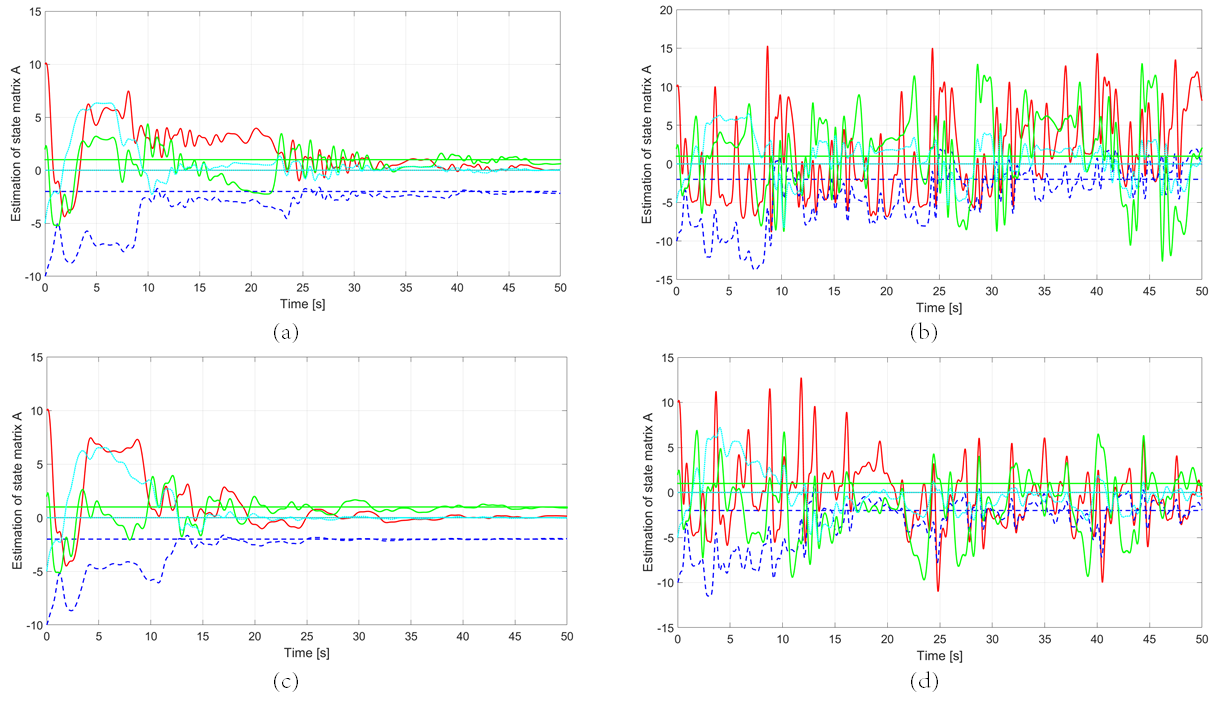
\includegraphics[width=.95\columnwidth]{figures/adaptive_A.png}
	\centering
	\caption{The adaptive estimation of the state matrix A, a. Without noise, b. With drift mass, c. With measurement noise, d. With measurement noise and drift mass.}
	\label{fig_adaptive_A}
\end{figure}

\begin{figure}[!h]
	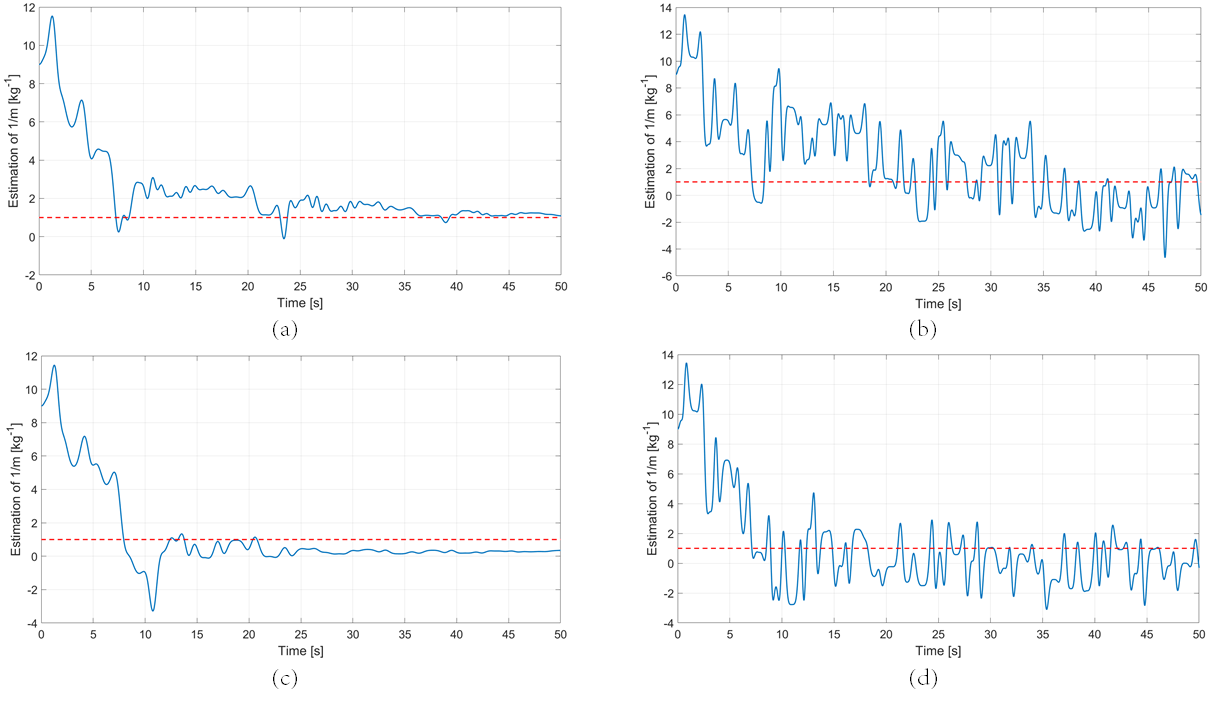
\includegraphics[width=1\columnwidth]{figures/adaptive_1_m.png}
	\centering
	\caption{The adaptive estimation of the fraction $\frac{1}{m}$, a. Without noise, b. With drift mass, c. With measurement noise, d. With measurement noise and drift mass.}
	\label{fig_adaptive_1_m}
\end{figure}

\begin{figure}[!h]
	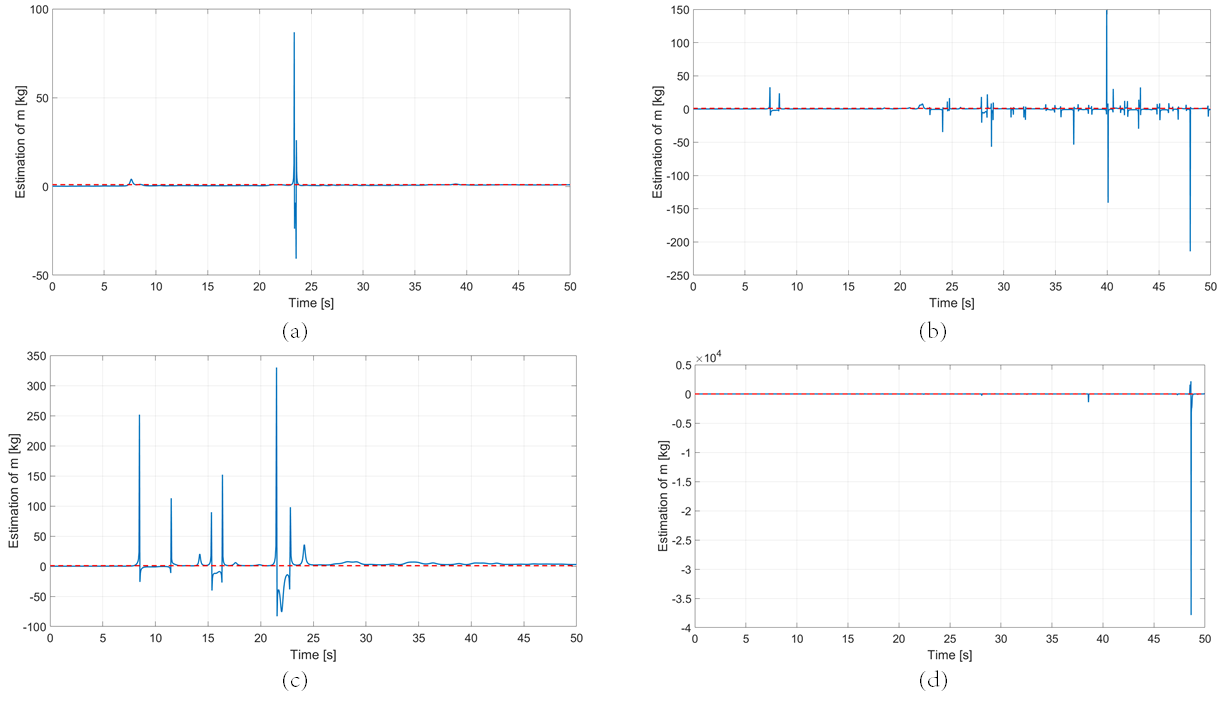
\includegraphics[width=.95\columnwidth]{figures/adaptive_m.png}
	\centering
	\caption{The adaptive estimation of the mass m, a. Without noise, b. With drift mass, c. With measurement noise, d. With measurement noise and drift mass.}
	\label{fig_adaptive_m}
\end{figure}

In Figure~\ref{fig_adaptive_A} the case with the measurement noise has the faster performance as we expected from a richer input with noise. When drift mass is imposed, the system oscillates because the state matrix $A$ becomes time-varying. In Figures~\ref{fig_adaptive_1_m}, \ref{fig_adaptive_m} the mass converges to the correct value for only the noise-free case, but still very slow. When measurement noise appears the mass converges again faster, but with an error. 

Comparing with the previous techniques the adaptive estimation algorithm is not sufficient to guarantee convergence to the correct value, unless we select a sufficiently rich input signal that will excite all the modes of the system. Moreover, the later approach relies on the stability of the system and the input $u$. For this reason we added a damping factor to the state matrix $A$, that makes our system stable.


\end{document}


